A fase 3 tem inicio com a utilização de técnicas automáticas para gerar artefatos multimídia a partir de modelos previstos. O Sistema consulta o plano de ação, e utiliza as informações contidas na base consolidada de contribuições para instanciar os artefatos multimídia definidos no plano de ação.  

\begin{figure}[ht]
\centering
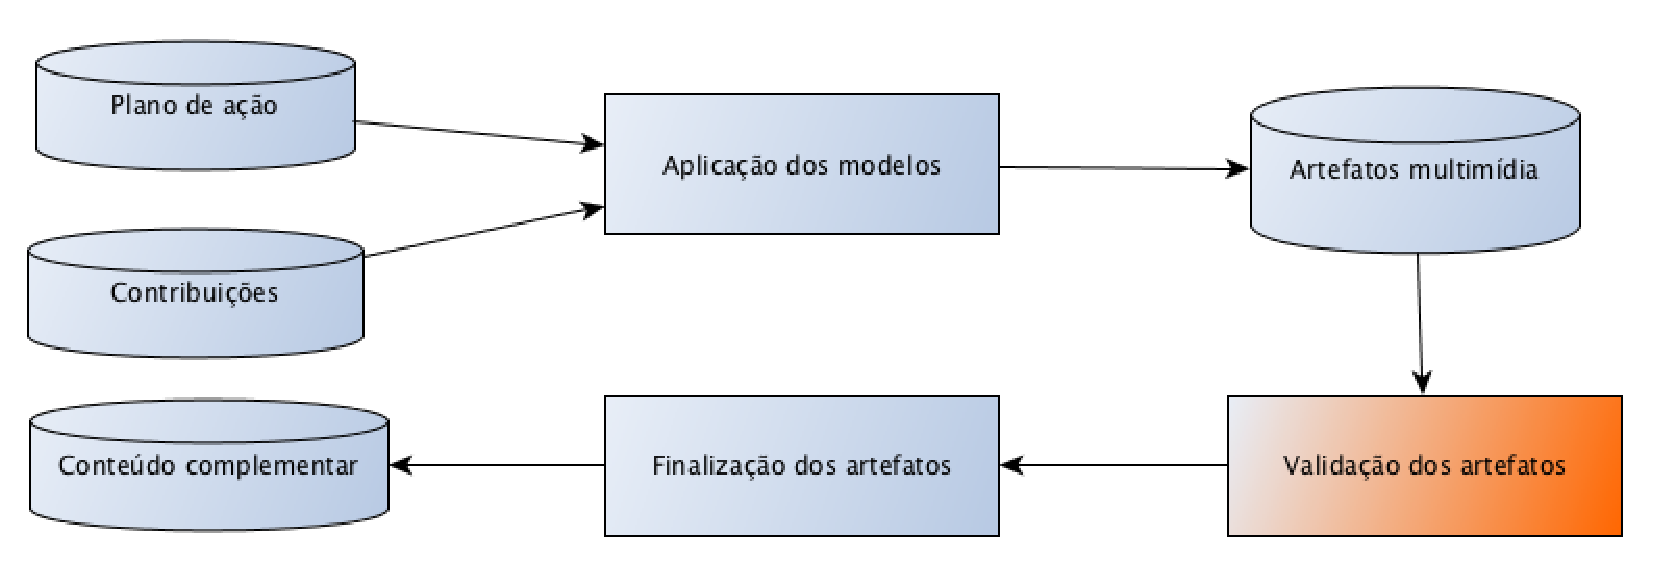
\includegraphics[width=.99\textwidth]{imagens/metodo/fase3_oa.eps}
\caption{Fase 3 do método}
\label{fig:metodo:fase3}
\end{figure}

Pode ser observado na Figura ~\ref{fig:metodo:fase3} que após gerados, os artefatos precisam ser validados. De acordo com o que foi definido no plano de ação, a validação pode ser feita pelo Iniciador, ou pelos Estudantes em uma abordagem semelhante a utilizada na fase 2. Uma vez validados, os artefatos são finalizados, ou seja, são formatados e adequados para serem agregados ao vídeo.

